\chapter[Directional detection]{Speed parametrisation for directional experiments}

\section{Introduction}

While traditional direct detection experiments seek to measure the recoil energies deposited by WIMPs scattering off detector nuclei, \textit{directional} experiments aim to measure both the energy and direction of the recoil. While the recoil distribution of typical backgrounds is expected to be roughly isotropic, the WIMP-induced recoil distribution is expected to be highly directional. The motion of the Sun through the Galactic DM halo generates a so-called `WIMP wind,' leading to an event rate peaked in the opposing direction, the direction of the constellation of Cygnus. 

The ability of directional detection to distinguish background from signal and to provide a model independent confirmation of the dark matter origin of the signal make it a promising search strategy. However, measuring the direction of rare, low energy recoils remains challenging \cite{}. A number of directional detectors are currently in development and a number of novel methods for directional detection have been proposed.

Measuring the directional recoil spectrum allows us to probe not only the energy distribution of WIMPs in the Galactic halo (embodied in the speed distribution $f(v)$), but the full 3-dimensional velocity distribution $f(\textbf{v})$. This may allow us to gain new insight into the formation processes at hand in the growth of the Milky Way halo \cite{}. However, it also introduces new uncertainty into calculating the event rate. While non-directional detection leaves us with a single free function in the form of  $f(v)$, the directional case relies upon the \textit{a priori} unknown function of a 3-dimensional vector, $f(\textbf{v})$.

In this chapter, we will first introduce the formalism by which the directional rate is calculated. Specifically, we introduce the Radon transform which relates the WIMP velocity distribution to the corresponding nuclear recoil distribution.  We then discuss the current state of directional detection technology and the progress of several directional experiments. We then discuss previous approaches to mitigating the uncertainties associated with the velocity distribution. Finally, we consider a new method for parametrising $f(\textbf{v})$, which allows it to be written in terms of a finite number of one-dimensional functions, and how to calculate the Radon transform of this new, discretised distribution function.

\section{Directional event rate}

First, we wish to calculate the directional event spectrum in a dark matter detector. We follow the treatment of Gondolo \cite{Gondolo:2002}, noting that similar calculations were performed previously by Copi, Heo and Krauss \cite{Copi:1999} and later by Copi and Krauss \cite{Copi:2002}. The scattering of a dark matter (DM) particle with a nucleus is illustrated in Fig.~\ref{fig:directional:scattering}. 

\begin{figure}[h!]
  \centering
  \includegraphics[width=0.75\textwidth]{Directional/Scattering.pdf}
\caption[Illustration of DM-nucleus scattering]{Illustration of the scattering of a DM particle of mass $m_\chi$ from a nucleus of mass $m_N$.}
  \label{fig:directional:scattering}
\end{figure}

We consider a DM particle of mass \(m_\chi\) impinging with velocity \(\textbf{v} = v\left(1,0\right)\) on a stationary target nucleus of mass \(m_N\). The dark matter scatters with velocity \(\textbf{v}' = v'\left(\cos \theta',\sin \theta'\right)\) and the nucleus scatters with final momentum \(\textbf{q} = q\left(\cos \theta, \sin \theta\right)\). From conservation of linear momentum we obtain:

\begin{align}
m_\chi v' \cos \theta' &= m_\chi v - q\cos \theta \,, \label{eq:momentumx}\\
m_\chi v' \sin \theta' &= q \sin \theta \,. \label{eq:momentumy}
\end{align}
We can eliminate \(\theta'\) by summing the squares of Eqs. \ref{eq:momentumx} and \ref{eq:momentumy}, to obtain:

\begin{equation}
v'^2 = v^2 - \frac{2 v q \cos \theta}{m_\chi} + \frac{q^2}{m_\chi^2}\,.
\end{equation}
From energy conservation, we obtain:

\begin{equation}
\label{eq:Energy}
v'^2 = v^2 - \frac{q^2}{m_\chi m_N} \,.
\end{equation}
Combining these, we see that the recoil momentum of the target nucleus is given by

\begin{equation}
\label{eq:constraint}
q = 2\mu_{\chi N} v \cos \theta \,,
\end{equation}
where \(\mu_{\chi N} = m_\chi m_N/(m_\chi + m_N)\) is the DM-nucleus reduced mass.


For a WIMP-nucleus interaction cross section which is independent of velocity, we can write the differential cross section as 

\begin{equation}
\frac{\textrm{d}\sigma}{\textrm{d}E_R} = \frac{m_N \sigma_p}{2 \mu_{\chi p}^2 v^2} \mathcal{C} F^2(E_R)\,,
\end{equation}
where \(E_R\) is the nuclear recoil energy, \(\sigma_p\) is the WIMP-proton interaction cross section (which may be spin-dependent (SD) or spin-independent (SI)) and $\mathcal{C}$ and $F^2$ are the corresponding enhancement factor and nuclear form factor (see Eq.~\ref{eq:DD:fullsigma}).

We now obtain from here the double differential cross-section \(\frac{\textrm{d}\sigma}{\textrm{d}E_R \textrm{d}\Omega_q}\). The collision is azimuthally symmetric, so that \(\textrm{d}\Omega_q = 2\pi\,\textrm{d}\cos\theta\). We then require a Dirac \(\delta\)-function to impose the condition in Eq.\ \ref{eq:constraint}: \(\delta\left(\cos\theta - q/2\mu_{\chi N}v\right) = v \delta\left(v \cos\theta - q/2\mu_{\chi N}\right)\). We finally obtain

\begin{equation}
\frac{\textrm{d}\sigma}{\textrm{d}E_R \textrm{d}\Omega_q} = \frac{m_N \sigma_p}{4\pi\mu_{\chi p}^2v} \mathcal{C} F^2(E_R) \delta\left(v \cos\theta - v_\textrm{min}\right)\,
\end{equation}
where \(v_\textrm{min}\) is the minimum WIMP speed required to excite a recoil of momentum \(q\) or, equivalently, energy \(E_R\):

\begin{equation}
v_\textrm{min} = \frac{q}{2\mu_{\chi N}} = \sqrt{\frac{m_N E_R}{2\mu_{\chi N}^2}}\,.
\end{equation}

To obtain the differential rate per unit detector mass, we divide by the mass of the target nucleus and multiply by the WIMP flux at velocity \(\textbf{v}\),

\begin{equation}
\frac{\rho_0}{m_\chi} v f(\textbf{v}) \, \textrm{d}^3 \textbf{v}\,,
\end{equation}
before integrating over all WIMP velocities, where \(\rho_0\) is the local dark matter mass density. Combining these, we obtain:

\begin{equation}
\frac{\textrm{d}R}{\textrm{d}E_R \textrm{d}\Omega_q} = \frac{\rho_0 \sigma_p}{4\pi \mu_{\chi p}^2 m_\chi} \mathcal{C} F^2(E_R) \hat{f}\left(v_\textrm{min},\hat{\textbf{q}}\right)\,,
\end{equation}
where \(\hat{f}\left(v_\textrm{min},\hat{\textbf{q}}\right)\) is the Radon Transform of the velocity distribution, defined as:

\begin{equation}
\hat{f}\left(v_\textrm{min},\hat{\textbf{q}}\right) = \int \delta\left(v_\textrm{min} - \textbf{v}\cdot\hat{\textbf{q}}\right) f(\textbf{v}) \,\textrm{d}^3\textbf{v}\,.
\end{equation}
Geometrically, this is the integral of \(f(\textbf{v})\) over a plane perpendicular to \(\hat{\textbf{q}}\) at a distance \(v_\textrm{min}\) from the origin. In physical terms, for a given recoil angle and energy, we integrate over all WIMP velocities satisfying the kinematic constraint given by Eq.\ \ref{eq:constraint}.

\subsection{Examples}

We consider several examples of velocity distributions and their corresponding Radon transforms. For an isotropic Maxwell-Boltzmann distribution with dispersion $\sigma_v$,

\begin{equation}
f(\textbf{v}) = \frac{1}{(2\pi \sigma_v^2)^{\frac{3}{2}}} \exp \left[ -\frac{\textbf{v}^2}{2 \sigma_v^2}\right]\,,
\end{equation}
the Radon transform is also isotropic,
\begin{equation}
\hat{f}(v_q,\hat{\textbf{q}}) = \frac{1}{(2\pi \sigma_v^2)^{\frac{1}{2}}} \exp \left[ -\frac{v_q^2}{2 \sigma_v^2}\right]\,.
\end{equation}
If we take this form to describe the DM velocity distribution in the galactic frame, we must transform to the laboratory frame using the relation \cite{Gondolo:2002}

\begin{equation}
\hat{f}_\textrm{lab}(v_q, \hat{\textbf{q}}) = \hat{f}_\textrm{gal}(v_q - \textbf{v}_\textrm{lag}\cdot\hat{\textbf{q}} , \hat{\textbf{q}})\,,
\end{equation}
where $\textbf{v}_\textrm{lag}$ is the velocity of the peak of the galactic distribution with respect to the laboratory. We therefore obtain the Radon transform of the Standard Halo Model

\begin{equation}
\label{eq:directional:SHM}
\hat{f}(v_q,\hat{\textbf{q}}) =  \frac{1}{(2\pi \sigma_v^2)^{\frac{1}{2}}} \exp \left[ -\frac{(v_q - \textbf{v}_\textrm{lag}\cdot\hat{\textbf{q}})^2}{2 \sigma_v^2}\right]\,.
\end{equation}
This can be extended to incorporate a cut off at the galactic escape velocity, or for more general anisotropic velocity distributions \cite{Gondolo:2002}.

Another interesting velocity distribution is that of a stream

\begin{equation}
f(\textbf{v}) = \delta(\textbf{v} - \textbf{v}_s)\,,
\end{equation}
which has Radon transform

\begin{equation}
\hat{f}(v_q,\hat{\textbf{q}}) =  \delta(v_q - \textbf{v}_\textrm{lag}\cdot\hat{\textbf{q}})\,.
\end{equation}
This results in a highly directional signal, producing a spherical recoil spectrum centred on $\textbf{v} = \textbf{v}_s/2$.

In Fig.~\ref{fig:directional:Radon}, we illustrate the Radon transform of the SHM (top), the SHM with a contribution from a dark disk (middle), and a stream (bottom). We evaluate the Radon transform at a value $v_q = 100 \kms$. In all cases, there is a clear anisotropy and the three scenarios are easily distinguishable. This highlights the discriminatory power of directional detection. It has previously been demonstrated that only of order 10 events would be required to distinguish a directional WIMP signal from an isotropic background. Furthermore, with of order 100 events, it should be possible to detect any deviation in peak recoil direction due to a stream \cite{Morgan:2005}.

\begin{figure}[h!]
  \centering
  \includegraphics[width=0.75\textwidth]{Directional/SHMradon.pdf}

  \includegraphics[width=0.75\textwidth]{Directional/DDradon.pdf}

  \includegraphics[width=0.75\textwidth]{Directional/STREAMradon.pdf}

\caption[Radon transform examples]{Radon transform of the SHM (top), SHM with a dark disk contribution (middle) and stream (bottom) distribution functions, evaluated at $v_q = 100 \kms$.}
  \label{fig:directional:Radon}
\end{figure}

\todo{Say more about DD}

\section{Directional experiments}
\label{sec:directional:experiments}
Directional experiments are still in the prototype stage, with detectors being around 1 $\textrm{m}^3$ in size, with hopes for a scale up to ton-scale experiments in the future. A number of experiments use time projection chamber (TPC) technology to achieve directional sensitivity. These include DRIFT \cite{Daw:2011,Daw:2012}, NEWAGE \cite{Miuchi:2010,Miuchi:2012}, MIMAC \cite{Riffard:2013, Santos:2013}, DMTPC \cite{Monroe:2012,Battat:2013} and D3 \cite{Vahsen:2012}.

In order to have directional sensitivity, a detector must image the tracks produced by the recoiling nucleus in the detector. The typical range of a WIMP-nucleus recoil is only $\sim$100nm, however, which makes track reconstruction difficult. Directional experiments therefore operate in the low pressure gas phase (around 0.05 atm \cite{Daw:2012}) in order to maximise the distance travelled by a recoiling nucleus. The detector is filled with a target gas such as $CF_4$ (in the case of the DRIFT experiment) which provides sensitivity to spin-dependent recoils. Nuclear recoils in the detector ionize the target gas. The freed electrons are drifted under an electric field to the faces of the detector where the charge is collected. Alternatively, an electron transport gas ($CS_2$ in the DRIFT experiment) may be added, which attracts the free electrons forming ions which are then collected. 

The energy of the recoil can be recovered from the total amount of ionisation in the event. The three dimensional track (which is only a few mm long) can be reconstructed from the distribution of charge detected at the surface of the detector volume, with information about the z-direction obtained from the timing of the charges arriving at the surface. \note{Check this...} This method allows an angular resolution of 20$\,^{\circ}$-80$\,^{\circ}$ using current prototypes \cite{Billard:2012}, with higher resolution at higher recoil energies. However, the sense of the recoil is much more difficult to determine, requiring sensitivity to tiny asymmetries between the start and end of the track. While sense discrimination has previously been demonstrated \cite{Burgos:2008}, it cannot be achieved with 100\% efficiency. Even for high energy (100 keV) recoils, studies suggest that only partial sense recognition may be possible (with only a 65\% probability of correctly determining the sense) \cite{Billard:2012}. Without sense discrimination the anisotropy of the WIMP signal is reduced and roughly 3 times more events are required to establish the directionality of the signal and distinguish from an anisotropic background \cite{Morgan:2005,Green:2008}.

\note{Talk about anodes rather than surfaces...}

\note{Background - Radon progeny; fiducialisation; thresholds}

A number of other directional technologies have also been suggested. Nuclear emulsion experiments use as a target silver halide crystals suspended in gelatin \cite{Naka:2012}. The emulsion required must be composed of very fine grains in order to image dark matter recoil tracks smaller than 1 $\mu \textrm{m}$, however angular resolutions below 20$\,^{\circ}$ may be achievable. DNA based experiments \cite{Drukier:2012} have also been proposed which may be able to achieve directional sensitivity. The main TPC-based experiments are in cooperation and are ultimately aiming to construct a ton-scale `CYGNUS' detector \cite{Ahlen:2009}.


\section{Reconstructing the velocity distribution}

With promising developments in directional detector technology, it is interesting to ask what information about the velocity distribution we could, in principle, extract from a directional signal. Alves, Hendri and Wacker \cite{Alves:2012} investigated the possibility of describing $f(\textbf{v})$ in terms of a series of special functions of integrals of motion (energy and angular momentum). These can then be fit to data, with around 1000 events required to distinguish between the SHM and a Via Lactea II distribution function \cite{Kuhlen:2008}. However, the special, separable form of the velocity distribution requires that the dark matter halo is in equilibrium. Moreover, this method requires an \textit{a priori} knowledge of the DM mass (for example from earlier non-directional detectors or from collider experiments).

A more general parametrisation for the velocity distribution was recently proposed by Lee \cite{Lee:2014}. In this approach, the velocity distribution is decomposed into products of Fourier-Bessel functions and spherical harmonics. This is completely general and does not require that the halo is completely virialised. Lee also gives an analytic expression for the Radon transform of the Fourier-Bessel basis, making this approach computationally efficient. However, this basis does not guarantee that the resulting $f(\textbf{v})$ is everywhere positive and therefore not all combinations of coefficients correspond to physical distribution functions. \note{Might be a good idea after a large number of events have been found...}

In fact, any decomposition in terms of spherical harmonics leads to this problem. It is unclear how this issue will affect parameter reconstruction. Without some criteria which determines which coefficients of the spherical harmonics lead to strictly positive distribution functions, it may be necessary to numerically test each parametrised distribution function for negative values. However, for a real function of three parameters $f(\textbf{v}) = f(v_x, v_y, v_z)$ this would require a very large number of evaluations, which may not be computationally feasible. In addition, it is not clear how this property would affect an exploration of the parameter space using, for example, Markov Chain Monte Carlo or Nested Sampling \cite{OrRefToSec}. Physical distribution functions may occupy only a small fraction of the total space of parameters or may be distributed over a large number of irregular regions in the parameter space, making sampling from them difficult.

In Sec.~\ref{sec:directional:discretising}, I will present an alternative method of parametrising the velocity distribution, which can guarantee that the velocity distribution is everywhere positive and therefore represents a promising and general method for extracting information from directional experiments. However, first it will be instructive to discuss the invertibility of the Radon transform. That is, given a perfect realisation of the directional recoil spectrum, can we perfectly reconstruct the corresponding velocity distribution.

\todo{Point out that this is harder when you have a full 3-D function...?}

\subsection{Invertibility of the Radon transform} 

\todo{Make sure to check and improve the terminology - especially `null functions'}

It has been shown that for distributions \(f(\textbf{v})\) which are rapidly decreasing at infinity \cite{Helgason:1999} or which are compactly supported \cite{Quinto:1983}, the Radon Transform is one-to-one and is therefore exactly invertible. This inversion is typically unstable (that is, the reconstructions are very sensitive to noise in the signal) and ill-posed (as not all functions are valid Radon Transforms). However, assuming that \(\hat{f}\) is a valid Radon Transform and that we have full knowledge of it, we can reconstruct $f(\textbf{v})$ exactly.

However, due to finite energy thresholds, we do not have access to the low-speed region of $\hat{f}(v_\textrm{min}, \hat{q})$. We must therefore consider the related Exterior Radon Transform \(\mathcal{R}_E\). Only using values of the Radon Transform for \(v_{\textrm{min}} > v_a\), is it possible to reconstruct $f(\textbf{v})$ for $v > v_a$? If \(f\) is rapidly decreasing at infinity, this transform is still one-to-one, as in the complete case. However, if \(f\) decays as an inverse power of \(v\) (i.e.\ \(f \sim v^{-k}\) as \(v\rightarrow \infty\)) the Exterior Transform is no longer one-to-one \cite{Shepp:1978}. \todo{Define null space...} In this case, the null space in 3 dimensions is non-trivial \cite{Quinto:1982}, consisting of functions of the form:

\begin{equation}
\label{eq:null}
f_N(\textbf{v}) = \frac{\alpha}{v^{3+k}} Y_{lm}(\hat{\textbf{v}}),
\end{equation}
where \(\alpha\) is some constant, \(Y_{lm}\) is a spherical harmonic, \(0 \leq k < l\) and \(l-k\) is even. This means that there are no null functions for \(l = 0\) or \(l = 1\). It can be shown by explicit calculation that such functions have a Radon Transform of zero for all \(v_\textrm{min} > 0\).

In the case of direct detection, the point at \(v = v_\textrm{min} = 0\) corresponds to DM particles at rest with respect to the detector, which can impart no recoil energy and are therefore undetectable. For directional detection then, even for infinitesimally small threshold energies, we must consider the Exterior Radon Transform.

This means that for a given Radon transform, adding any combination of functions of the form $f_N(\textbf{v})$ to $f(\textbf{v})$ leads to the same Radon transform. However, we note that the spherical harmonics with \(l > 0\) can take negative values. However, at large values of \(v\), \(f_\textrm{SHM}\) decays exponentially. By contrast, \(f_N\) decays as a power of \(v\), meaning at some (potentially large) value of \(v\) the magnitude of the null function will exceed that of \(f(\textbf{v})\) leading to a negative distribution function. A more general distribution function will have a natural cut-off (say at the galactic escape speed) and will certainly decay rapidly to zero for high values of \(v\). As a result, we can neglect the impact of null functions on reconstructions.

Thus, as long as we choose basis functions which are everywhere positive and therefore physically valid, we ensure that the Radon transform is invertible. This means that no information is lost in reconstructing $f(\textbf{v})$ and also that there are no unphysical degeneracies present in the parametrisation we have chosen.

\todo{NB: Make it very clear that if we choose a parametrisation which can be somewhere negative (even if it's a high energies where these things don't matter because its above threshold and only a small effect), it can lead to problems of non-invertibility and introduce unphysical degeneracies in the parametrisation. Therefore it is very important to make sure that $f(\textbf{v})$ is everywhere positive. I should include some plots of the null functions and of truncated null functions (added to $f(\textbf{v})$) to indicate what can go wrong - and how bad things can be. Also, talk about truncated null functions and check that if we ensure positive-definiteness then truncated null functions shouldn't cause a problem... Double-check to see if truncated null functions (truncated at the same place as the full distribution function) are still null (they shouldn't be, don't just look along one direction, but all... IT DEFINITELY IS NOT NULL, SO THAT'S FINE...)}

\note{Also say that I don't think that this has previously been discussed...}

\section{Discretising the velocity distribution}
\label{sec:directional:discretising}

In order to ensure that the velocity distribution is everywhere positive, we propose an alternative methodology. We propose that the velocity distribution be discretised into $N$ angular components, each described by a single function of the WIMP speed:

\begin{equation}
f(\textbf{v}) = f(v, \cos\theta', \phi') =
\begin{cases}
f_1(v) & \textrm{ for } \theta' \in \left[ 0, \pi/N\right]\,, \\
f_2(v) & \textrm{ for } \theta' \in \left[ \pi/N, 2\pi/N\right]\,, \\
 & \vdots\\
f_k(v) & \textrm{ for } \theta' \in \left[ (k-1)\pi/N, k\pi/N\right]\,, \\
 & \vdots\\
f_N(v) & \textrm{ for } \theta' \in \left[ (N-1)\pi/N, \pi\right]\,. \\
\end{cases}
\end{equation}
We consider for simplicity only a discretisation in $\cos\theta'$, though this can be extended to an additional discretisation in $\phi'$ if required. 


The motivation for this description is that the simplest signal (beyond an isotropic $N=1$ signal) which can be observed with a directional detectors is a discrete asymmetry (between the event rates in, say, the forward and backward directions). Shortly after the confirmation of a dark matter signal at a directional detector, the number of events may still be quite small (for example, the roughly 10 events required to distinguish from an isotropic background). In this small statistics scenario, constraining a large number of free functions is not feasible. However, if we discretise $f(\textbf{v})$ into $N=2$ angular components, it should be possible to extract some meaningful directional information with only a small number of events. With larger numbers of events, $N$ can be increased to allow more directional information to be extracted. \note{Improve justification...}

Because angular information is being lost from the velocity distribution, we cannot consider using the full Radon transform to constrain the functions $f_k(v)$, as this contains additional angular information. Instead, we should consider integrated Radon transforms of the form:

\begin{equation}
\hat{f}_k(v_\textrm{min}) = \int_{\phi = 0}^{2\pi} \int_{(k-1)\pi/N}^{k\pi/N} \hat{f}(v_\textrm{min}, \hat{\textbf{q}})\, \mathrm{d}\cos\theta\mathrm{d}\phi,
\end{equation}
 where $\hat{\textbf{q}} = (\cos\theta, \phi)$. Thus, we will be using a discretised version of the Radon transform (or equivalently, the event rate and, ultimately, data) in order to constrain the functional form of a discretised velocity distribution. \note{Improve this justification and/or swap this paragraph with the one before it...}

What form should be used for the free functions $f_k(v)$? This discretisation scheme does not depend on choosing a particular form for the $v$ dependence of the velocity distribution. We can therefore choose any parametrisation for $f_k(v)$ - such as those described in Sec.~\ref{somesections} - having convinced ourselves that they introduce no bias into the fitting procedure. The question we will address here is what \textit{angular} errors are introduced by such a discretisation. We will now demonstrate for the cases of $N=1, 2, 3$ how the corresponding Radon transform is calculated and how it compares to the true Radon transform for some benchmark cases.

\todo{Talk somewhere about tomography...}

\subsection{$N=1$ discretisation}

The $N=1$ case corresponds to the assumption that $f(\textbf{v})$ is isotropic. That is, we could consider setting $f(\textbf{v})$ equal to its angular average:  $f(\textbf{v}) = \bar{f}(v) \equiv \frac{1}{4\pi} \int f(\textbf{v}) \, \mathbf{d}\Omega_v$. The Radon transform then reduces to

\begin{equation}
\label{eq:directional:radonN1}
\hat{f}\left(v_\textrm{min},\hat{\textbf{q}}\right) = \int \delta\left(v_\textrm{min} - \textbf{v}\cdot\hat{\textbf{q}}\right) \bar{f}(v) \,\textrm{d}^3\textbf{v}\,.
\end{equation}

We can rewrite the delta function as

\begin{equation}
\delta\left(v_\textrm{min} - \textbf{v}\cdot\hat{\textbf{q}}\right) = \frac{1}{v}\delta(v_\textrm{min}/v - \hat{\textbf{v}}\cdot\hat{\textbf{q}})\,, 
\end{equation}
which means that Eq.~\ref{eq:directional:radonN1} becomes  

\begin{equation}
\hat{f}\left(v_\textrm{min},\hat{\textbf{q}}\right) = \int_{v=0}^\infty \frac{v^2\bar{f}(v)}{v} \oint \delta\left(v_\textrm{min}/v - \hat{\textbf{v}}\cdot\hat{\textbf{q}}\right)  \, \mathrm{d}\Omega_v\mathrm{d}v\,.
\end{equation}
The angular integral evaluates to unity as long as $v_\textrm{min}/v = \hat{\textbf{v}}\cdot\hat{\textbf{q}}$ for some value of $\hat{\textbf{v}}$ in the domain of integration. Because we integrate over all directions $\hat{\textbf{v}}$, this is guaranteed to be satisfied for some value, as long as $v > v_\textrm{min}$ (because $\hat{\textbf{v}}\cdot\hat{\textbf{q}}$ cannot exceed unity). Thus,

\begin{equation}
\oint \delta\left(v_\textrm{min}/v - \hat{\textbf{v}}\cdot\hat{\textbf{q}}\right)  \, \mathrm{d}\Omega_v = \Theta(v - v_\textrm{min})\,,
\end{equation}
and
\begin{equation}
\hat{f}\left(v_\textrm{min},\hat{\textbf{q}}\right) = \int_{v=v_\textrm{min}}^\infty \frac{v^2\bar{f}(v)}{v} \mathrm{d}v\,.
\end{equation}

Finally, to obtain the directionally averaged Radon transform $\hat{f}(v_\textrm{min})$, we integrate over all directions $\qhat$. As the Radon transform is isotropic in this case, this gives a contribution of $4\pi$. Replacing the expression for $\bar{f}(v)$ with the directionally averaged velocity distribution, we therefore obtain \note{What should I call the directionally averaged RT?}

\begin{equation}
\hat{f}\left(v_\textrm{min}\right) = \int_{v=v_\textrm{min}}^\infty \frac{f(\textbf{v})}{v} \mathrm{d}^3\textbf{v}\,.
\end{equation}

This matches the expression for the total non-directional scattering rate. While we assumed here that $f(v)$ was isotropic, in first deriving this expression in Chapter~\ref{sec:DD}, no such assumption was required \note{Was it?}. We therefore see that in the $N=1$ case, the angular-discretised `approximation' is in fact exact and leads to the correct angular-averaged Radon transform.

\subsection{$N=2$ discretisation}

For the $N=2$ case, we are considering a forward-backward asymmetry in the velocity distribution:

\begin{equation}
\label{eq:directional:N2}
f(\mathbf{v}) =
\begin{cases}
f_1(v) & \textrm{if } \theta' \in [0, \pi/2] \\
f_2(v) & \textrm{if } \theta' \in [\pi/2, \pi]\,.
\end{cases}
\end{equation}

From these, we wish to obtain the integrated recoil spectra for the forward and back directions. Specifically:

\begin{align}
\hat{f}_1 &= \int_{0}^1 \hat{f}(v_q,\cos\theta) \, \mathrm{d}\cos\theta \\
\hat{f}_2 &= \int_{-1}^0 \hat{f}(v_q, \cos\theta) \, \mathrm{d}\cos\theta \,.
\end{align}
We will focus on the first of these, $\hat{f}_1$, as the other can be obtained simply by exchanging which directions are forward and backward (that is, by interchanging $f_1$ and $f_2$). From now on, we will therefore be working under the assumption that $\cos\theta \in [0,1]$.

We first consider calculating the azimuthally averaged Radon transform:

\begin{align}
\hat{f}(v_q, \cos\theta) &= \int_0^{2\pi} \hat{f}(v_q, \cos\theta, \phi) \, \mathrm{d}\phi \\
&= \int_0^{2\pi}\left( \int_{\mathbb{R}^3} f(\mathbf{v}) \delta\left(\mathbf{v}\cdot\hat{\mathbf{q}} - v_q \right)\, \mathrm{d}^3\mathbf{v} \right) \mathrm{d}\phi \\
&= \int_{\phi = 0}^{2\pi} \int_{v = 0}^{\infty} \oint v f(\textbf{v}) \delta\left(v_\textrm{min}/v - \hat{\textbf{v}}\cdot\hat{\textbf{q}}\right) \, \mathrm{d}\Omega_v \mathrm{d}v \mathrm{d}\phi\,.
\end{align}
We focus on performing the $\phi$ integral, which we define as:

\begin{align}
I(v_q, \cos\theta, \mathbf{v}) &= \int_{0}^{2\pi} \delta\left(\sin\theta\sin\theta' \cos(\phi-\phi') + \cos\theta\cos\theta' - v_q/v\right) \label{eq:defI} \, \mathrm{d}\phi \\
&\equiv \int_{0}^{2\pi} \delta\left(g(\phi)\right) \, \mathrm{d}\phi\,.
\end{align}
We then rewrite the delta function as a function of $\phi$:
\begin{equation}
\label{eq:deltadecomp}
\delta\left(g(\phi)\right) = \sum_{i} \frac{\delta(\phi - \phi_i)}{|g'(\phi_i)|}\,.
\end{equation}
Here, we sum over those values of $\phi_i$ satisfying $g(\phi_i) = 0$. We leave the details of the full calculation to Appendix~\ref{sec:appendix}. However, we obtain,

\begin{equation}
I(v_q, \cos\theta, \mathbf{v}) = \frac{2 C(\alpha)}{\sqrt{\left(\sin\theta\sin\theta'\right)^2 - \left(\beta - \cos\theta\cos\theta'\right)^2}}\Theta(v - v_q)\,,
\end{equation}
where
\begin{equation}
\beta = v_q/v\,; \qquad \alpha = \frac{\beta - \cos\theta\cos\theta'}{\sin\theta \sin\theta'}\,,
\end{equation}
and $C(\alpha) = 1$ for $\alpha \in [-1,1]$ and vanishing otherwise.

We therefore obtain

\begin{equation}
\hat{f}(v_q, \cos\theta) = \int_{v=v_q}^{\infty} \int_{\cos\theta=-1}^{1} \int_{\cos\theta'=-1}^{1} f(v, \cos\theta') I(v_q, \cos\theta, v, \cos\theta')\, v \mathrm{d}v \mathrm{d}\cos\theta \mathrm{d}\cos\theta'\,,
\end{equation}
with
\begin{equation}
f(v, \cos\theta') = \int_{0}^{2\pi} f(v, \cos\theta', \phi') \, \mathrm{d}\phi'\,.
\end{equation}

\note{Leave a load of the details for the appendix}

In the $N=2$ case, we obtain

\begin{align}
\label{eq:directional:N2result}
\hat{f}_1 &= 4\pi\int_{v_q}^{\infty} v \left( \pi f_1(v) + \atan\left\{\frac{\sqrt{1-\beta^2}}{\beta}\right\}\left(f_2(v) - f_1(v)\right) \right) \, \mathrm{d}v \\
\hat{f}_2 &= 4\pi\int_{v_q}^{\infty} v \left( \pi f_2(v) + \atan\left\{\frac{\sqrt{1-\beta^2}}{\beta}\right\}\left(f_1(v) - f_2(v)\right) \right) \, \mathrm{d}v\,.
\end{align}
We have also checked using Monte Carlo calculations that these are the correct forms of the forward and backward averaged Radon transforms in the case of a discretised velocity distribution.

We now wish to compare these approximate Radon transforms with the Radon transforms obtained from the full (non-discretised) velocity distribution. To do this, we select a benchmark velocity distribution (such as the SHM) and calculate $f_{1,2}$ according to Eq.~\ref{eq:directional:N2} by averaging over the $\cos\theta'$ in the forward and backward directions. This discretised velocity distribution is shown in Fig.~\ref{fig:directional:fN2}. We then insert these into Eq.~\ref{eq:directional:N2result} to obtain the forward and backward Radon transform. For comparison, we use the full velocity distribution of Eq.~\ref{eq:directional:SHM} to obtain the \textit{true} forward and backward Radon transforms by integrating over $\cos\theta$. 


\begin{figure}[t]
\label{fig:directional:fN2}
  \centering
  \includegraphics[width=1\textwidth]{Directional/SHMpolar.pdf}

  \includegraphics[width=1\textwidth]{Directional/SHMpolarN2.pdf}

\caption[Discretised velocity distribution for $N=2$ components]{Polar plots in $(v,\theta')$ for two velocity distributions. Shown are the SHM velocity distribution for $v_\textrm{lag} = 220 \kms$ and $\sigma_v = 156 \kms$ (top) and the discretised SHM distribution obtained by averaging in the forward and backward directions (bottom). The vector $\textbf{v}_\textrm{lag}$ is aligned along $\theta' = 0$. Note the different color scales in the two plots. \note{Put in units!!!}}
\end{figure}


The results of this comparison for a SHM model with $v_\textrm{lag} = 220 \kms$ and $\sigma_v = 156 \kms$ are shown in Fig.~\ref{fig:directional:radonN2}. While the general features are reproduced, there are some discrepancies. In particular, the forward Radon transform obtained using the approximate method is roughly 80\% of the correct result, while the backward Radon transform is up to 100\% larger using the approximate method. The reason for this is clear from Fig.~\ref{fig:directional:fN2}, which shows that the discretised velocity distribution has a greater fraction of WIMPs with velocities at right angles to the forward direction ($\theta' = 0$). Thus, the discretised velocity distribution has a greater chance of producing scatters in the backward direction. Overall, the discretised distribution is less focused in the forward direction, resulting in a reduced asymmetry between the forward and backward scattering rates. 

\begin{figure}[t]
\label{fig:directional:radonN2}
  \centering
  \includegraphics[trim={2cm 8cm 2cm 8cm},clip,width=0.80\textwidth]{Directional/N2-forward.pdf}

  \includegraphics[trim={2cm 8cm 2cm 8cm},clip,width=0.80\textwidth]{Directional/N2-backward.pdf}

\caption[True and approximate Radon transforms for $N=2$ components]{True and approximate forward and backward radon transforms when the full velocity distribution is discretised into N = 2 directional pieces. \note{Finish}}
\end{figure}



These discrepancies between the true and approximate recoil spectra may prove problematic when this method is employed in parameter estimation and the reconstruction of $f(\textbf{v})$. However, these discrepancies should be redued when the finite angular resolution of detectors is taken into account. \todo{Mention finite angular resolution...Do some plots...}

\todo{Consider a more radical distribution - such as a stream and show that it doesn't work so well...}

\subsection{$N=3$ discretisation}

Given the discrepancies in the $N=2$ case, we will now consider the $N=3$ discretisation, which should improve the fit between the true and approximate distribution. In addition, the $N=3$ will allow us to employ this methodology to the case where sense discrimination of recoils is not possible. Without sense discrimination, the forward and backward directions cannot be distinguished and the $N=2$ discretisation provides no directional sensitivity. As we shall see shortly, directional sensitivity is possible in the $N=3$ case.

We write the velocity distribution in discretised form as

\begin{equation}
\label{eq:directional:N3}
f(\mathbf{v}) =
\begin{cases}
f_1(v) & \textrm{if } \theta' \in [0, \pi/3] \\
f_2(v) & \textrm{if } \theta' \in [\pi/3, 2\pi/3] \\
f_3(v) & \textrm{if } \theta' \in [2\pi/3, \pi]\,.
\end{cases}
\end{equation}

If we interpret this discretisation as an averaging of the underlying velocity distribution, as before, we obtain the distribution in the bottom panel of Fig.~\ref{fig:directional:fN3} (the full SHM distribution is shown in the top panel for reference). Following the same procedure as for the $N=2$ case, we can obtain the corresponding forward, backward and transverse Radon transforms. The exact form of these is complicated (and not particularly instructive). However, this form can be generated using the algorithm described in Sec.~\ref{}, in which we treat the case of general $N$. 

\begin{figure}[t]
\label{fig:directional:fN3}
  \centering
  \includegraphics[width=1\textwidth]{Directional/SHMpolar.pdf}

  \includegraphics[width=1\textwidth]{Directional/SHMpolarN3.pdf}

\caption[Discretised velocity distribution for $N=3$ components]{Polar plots in $(v,\theta')$ for two velocity distributions. Shown are the SHM velocity distribution for $v_\textrm{lag} = 220 \kms$ and $\sigma_v = 156 \kms$ (top) and the discretised SHM distribution obtained by averaging in the forward, backward and transverse directions (bottom). The vector $\textbf{v}_\textrm{lag}$ is aligned along $\theta' = 0$. Note the different color scales in the two plots.}
\end{figure}

Again, we wish to test how closely the $N=3$ discretised distribution can reproduce the true forward-, backward- and transverse-averaged Radon transforms. The results are shown in Fig.~\ref{fig:directional:radonN2}. Compared to the $N=2$ case, the recoil spectra are reproduced much more closely, with a discrepancy of at most 15\% \note{check} between the true and approximate distributions.

\note{Emphasise that we haven't included the form factors...}

\begin{figure}[t]
\label{fig:directional:radonN3}
  \centering
  \includegraphics[trim={2cm 8cm 2cm 8cm},clip,width=0.80\textwidth]{Directional/N3-forward.pdf}

  \includegraphics[trim={2cm 8cm 2cm 8cm},clip,width=0.80\textwidth]{Directional/N3-backward.pdf}

  \includegraphics[trim={2cm 8cm 2cm 8cm},clip,width=0.80\textwidth]{Directional/N3-transverse.pdf}

\caption[True and approximate Radon transforms $N=3$ components]{True and approximate transforms when the full velocity distribution is discretised into N = 3 directional pieces. In the `forward' case $\cos\theta \in [1/2,1]$, in the `backward' case $\cos\theta \in [-1, -1/2]$, and in the `transverse case' $\cos\theta \in [-1/2, 1/2]$.}
\end{figure}

\subsubsection{The folded distribution}

As discussed in Sec.~\ref{sec:directional:experiments}, sense discrimination between forward and backward-going recoils may not be possible with near-future detectors. In this case then, all that can be measured is the so called `folded' recoil spectrum

\begin{equation}
\frac{\mathrm{d}R}{\mathrm{d}E_R\mathrm{d}|\cos\theta|} = \frac{\mathrm{d}R}{\mathrm{d}E_R\mathrm{d}\cos\theta} + \frac{\mathrm{d}R}{\mathrm{d}E_R\mathrm{d}(-\cos\theta)}\,.
\end{equation}
As a result, we are concerned not will the full Radon transform of $f(\textbf{v})$, but the folded Radon transform $\hat{f}(v_q, |\cos\theta|)$. In the case of $N=2$ discretisation, this folded Radon transform would have no directional information (because the forward and backward scattering rates differ only in the sign of $\cos\theta$). However, in the $N=3$ case, the transverse Radon transform, given by \note{define this earlier in the text...}

\begin{equation}
\hat{f}_T(v_q) = \hat{f}_2(v_q) = \int_{-1/2}^{1/2} \hat{f}(v_q, \cos\theta) \,\mathrm{d}\cos\theta\,,
\end{equation}
is invariant under $\hat{f}(v_q, \cos\theta) \rightarrow \hat{f}(v_q, |\cos\theta|)$ (apart from an overall factor of 2). That is, the transverse event rate `folds' back onto itself. Thus, even without sense discrimination, directional experiments will still be sensitive to this transverse scattering rate. By comparison, if the forward and backward directions cannot be distinguished, the remaining two averaged Radon transforms (the top two panels in Fig.~\ref{fig:directional:radonN3}) are folded together, to obtain the longitudinal rate
\begin{equation}
\hat{f}_L(v_q) = \int_{-1}^{-1/2} \hat{f}(v_q, \cos\theta) \,\mathrm{d}\cos\theta + \int_{1/2}^{1} \hat{f}(v_q, \cos\theta) \,\mathrm{d}\cos\theta\,.
\end{equation}

We plot the transverse and longitudinal averaged in Fig.~\ref{fig:directional:radonN3folded}. \note{Need a factor of 2 in the transverse bit...?} As expected, the two rates are now more similar in shape as we have lost some directional information. The approximate Radon transforms, obtained from the discretisation, match the true transforms closely for speeds above $v_q\approx 200 \kms$. \note{Why the discrepancy at low $v$?} For realistic experiments, these low speeds will be below the threshold energy of the experiment and the bias introduced by this discrepancy should be minimal \note{find some numbers for this...}. 

\begin{figure}[t]
\label{fig:directional:radonN3folded}
  \centering
  \includegraphics[trim={2cm 8cm 2cm 8cm},clip,width=0.80\textwidth]{Directional/N3-longitudinal.pdf}

  \includegraphics[trim={2cm 8cm 2cm 8cm},clip,width=0.80\textwidth]{Directional/N3-transverse.pdf}

\caption[True and approximate folded Radon transforms for $N=3$ components]{True and approximate folded transforms when the full velocity distribution is discretised into N = 3 directional pieces. In the `longitudinal' case $|\cos\theta| \in [1/2,1]$ while in the `transverse case' $|\cos\theta| \in [0, 1/2]$.}
\end{figure}

We note that in this folded case, we would fit to two functions, corresponding to the longitudinal and transverse event rates. However, our original discretisation required 3 free functions of $v$: $f_{1,2,3}(v)$. However, due to the properties of the Radon transform \note{(which are...?)}, the longitudinal rate is not a function of $f_1(v)$ and $f_3(v)$ but of the sum $f_1(v) + f_3(v) \equiv f_L(v)$. Thus, we have only two free functions to fit $f_{L,T}(v)$. 

\todo{-Fix captions on figures...}

\todo{-Discuss a dark disk case...}

\todo{-Discuss the poorly aligned - off axis case...}

\section{Discretisation for general $N$}

The procedure which has been described above can be extended to any number $N$ of angular bins. Significantly, for any value of $N$, the resulting Radon transform remains a sum of elementary, analytic functions multiplied by one dimensional functions $f_k(v)$. This means that no angular integration must be performed in order to obtain the Radon transform and at most $N$ one-dimensional integrals over the velocity $v$ must be performed, one for each of the $\hat{f}_k(v_q)$. 

While the details of the calculation can be found in Appendix~\ref{app}, we show below the full algorithm for calculating the averaged Radon transforms from a velocity distribution discretised into $N$ angular pieces...

\note{FINISH}

\section{Conclusion}

\todo{Check consistency with vmin and vq..., be careful about f's with subscript 1}
\todo{Check notation consistency with lefts( and rights)}
\note{We can even combine this with the non-directional experiments...}
